% !TeX root = ../thoulon_phd_defense_2025.tex
% \documentclass[../thoulon_phd_defense_2025.tex]{subfiles}
\documentclass[beamer]{standalone}

% \graphicspath{{\subfix{../chapters/}}}

\begin{document}
\section{Annexes}
\begin{frame}%[label=fra:gamma]
    \label{fra:gamma}
    \frametitle{$\Gamma$ function}

    \begin{figure}
    \centering
    \resizebox{!}{.7\textheight}{\subimport{resources/appendix/}{graph-gammad.tex}}
    \caption*{Plot of the $\Gamma$ function}
    \end{figure}

    \hyperlink{eq:gamma-bidis}{\beamerbutton{Back to cost and constraints}}
    \hyperlink{eq:gamma-bem}{\beamerbutton{Back to cost and constraints}}

\end{frame}

\begin{frame}
    \frametitle{The PTD extension}
\end{frame}


\subsection{Aerodynamics}
\begin{frame}
    \frametitle{RANS}
\end{frame}

\begin{frame}
    \frametitle{The aerodynamic adjoint}
\end{frame}

\subsection{BEM additional results}
\begin{frame}[plain]
    \label{fra:iter_adj_62}
    \begin{figure}
		\centering
		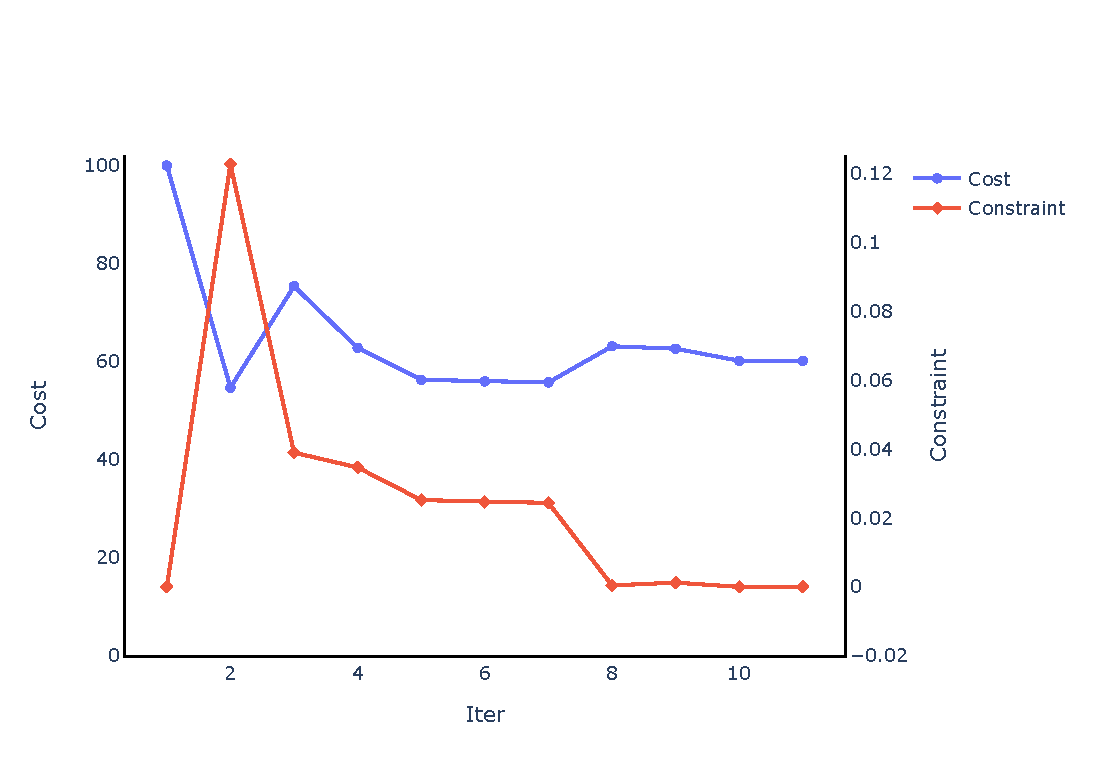
\includegraphics[trim=0 1cm 0 2.5cm, clip, width=1.\textwidth, right]{images/bem/iter_adj_62.pdf}
		\caption*{Adjoint BEM.}
	\end{figure}
    \hyperlink{fra:history-bem}{\beamerbutton{Back}}
\end{frame}

\begin{frame}[plain]
    \label{fra:iter_DF2_61}

	\begin{figure}
		\centering
		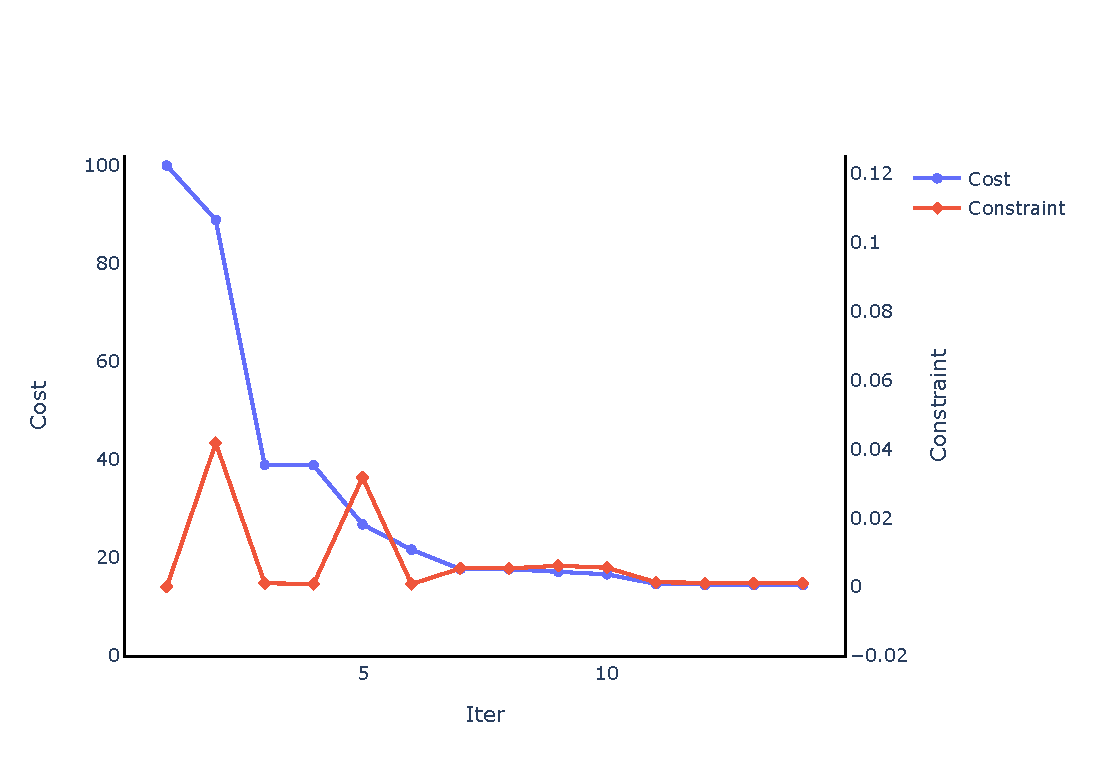
\includegraphics[trim=0 1cm 0 2.5cm, clip, width=1.\textwidth, right]{images/bem/iter_DF2_61.pdf}
		\caption*{FD BEM.}
	\end{figure}
    \hyperlink{fra:history-bem}{\beamerbutton{Back}}

\end{frame}

\begin{frame}[plain]
    \label{fra:iter_PTD_exact_100}
	\begin{figure}
			\centering
		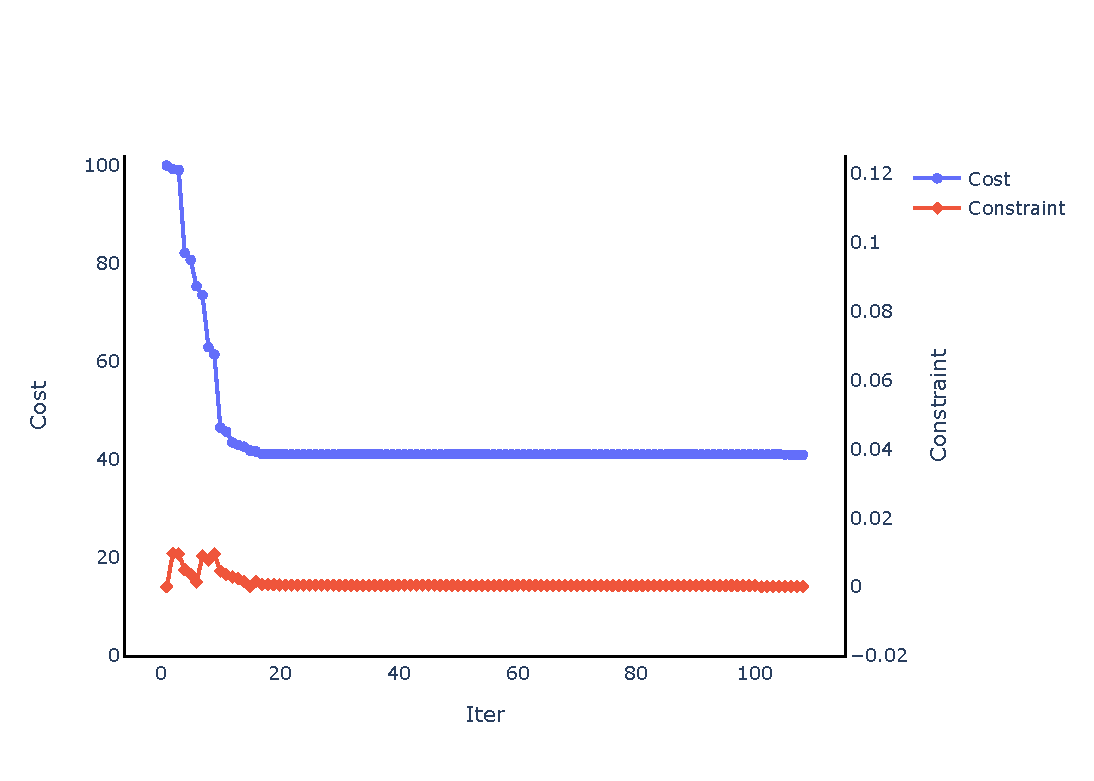
\includegraphics[trim=0 1cm 0 2.5cm, clip, width=1.\textwidth, right]{images/bem/iter_PTD_exact_100.pdf}
			\caption*{PTD with exact gradient.}
	\end{figure}
    \hyperlink{fra:history-bem}{\beamerbutton{Back}}
\end{frame}

\begin{frame}[plain]
    \label{fra:RCS_adj_62}
    \begin{figure}
		\centering
		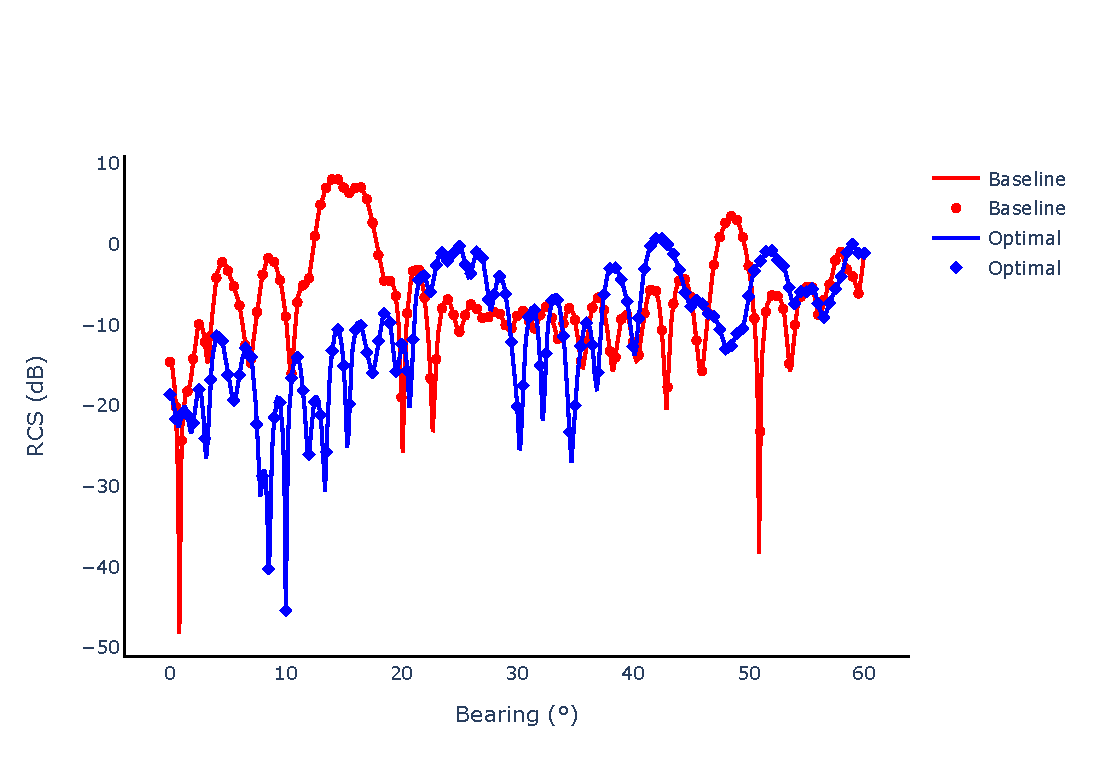
\includegraphics[trim=0 .8cm 0 2.5cm, clip, width=1.\textwidth]{images/bem/RCS_adj_62.pdf}
		\caption*{Adjoint BEM.}
	\end{figure}
    \hyperlink{fra:rcs-result-bem}{\beamerbutton{Back}}
\end{frame}

\begin{frame}[plain]
    \label{fra:RCS_DF2_61}

	\begin{figure}
		\centering
		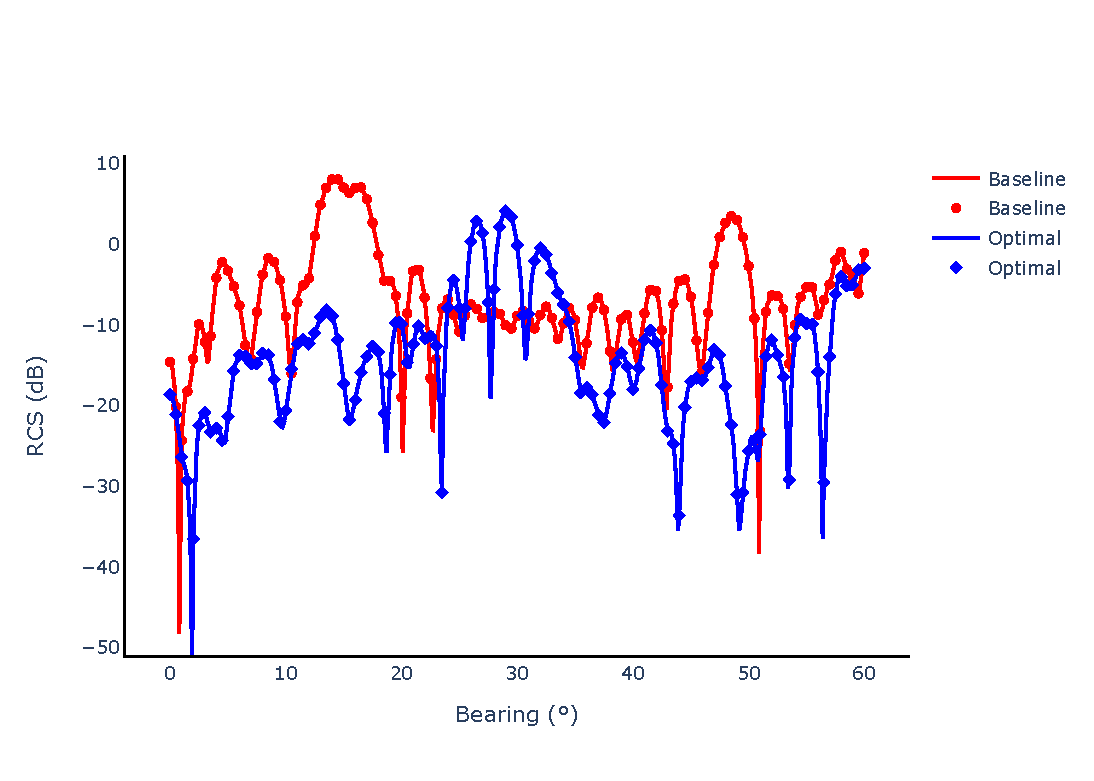
\includegraphics[trim=0 .8cm 0 2.5cm, clip, width=1.\textwidth]{images/bem/RCS_DF2_61.pdf}
		\caption*{FD BEM.}
	\end{figure}
    \hyperlink{fra:rcs-result-bem}{\beamerbutton{Back}}

\end{frame}

\begin{frame}[plain]
    \label{fra:RCS_PTD_exact_100}
	\begin{figure}
			\centering
			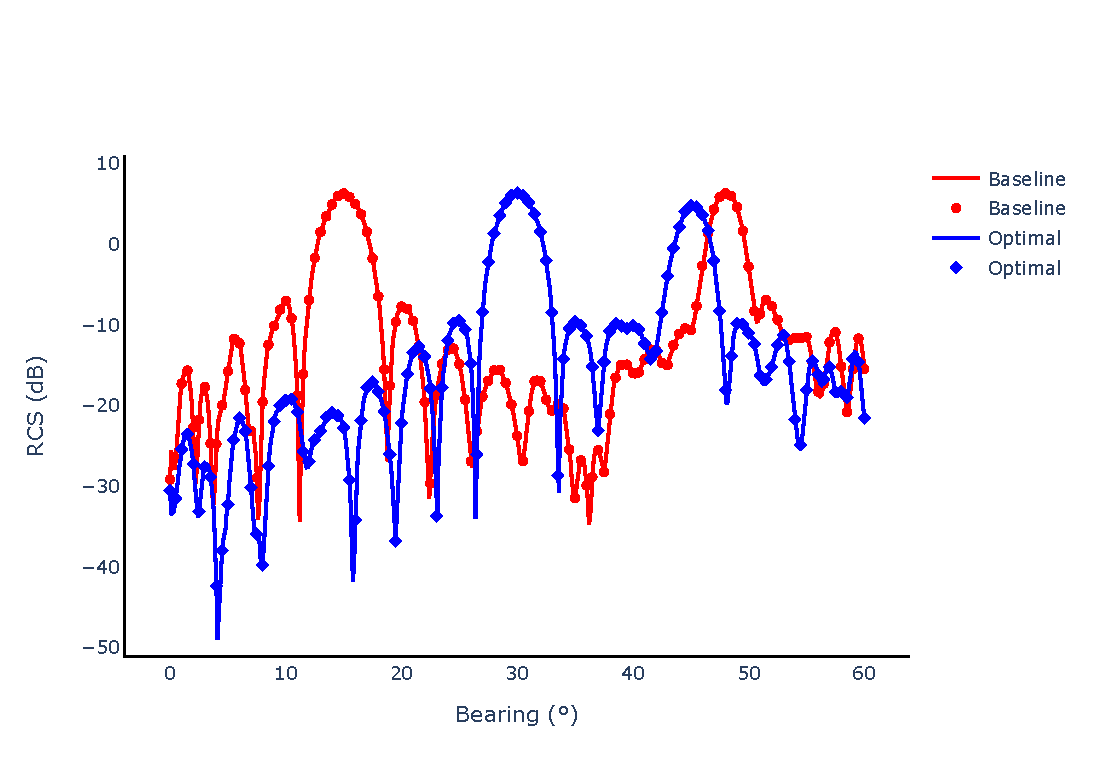
\includegraphics[trim=0 .8cm 0 2.5cm, clip,width=1.\textwidth]{images/bem/RCS_PTD_exact_100.pdf}
			\caption*{PTD with exact gradient.}
	\end{figure}
    \hyperlink{fra:rcs-result-bem}{\beamerbutton{Back}}
\end{frame}

\end{document}
